\section{HiTechnic NXT Compass Sensor}
Kompasset fra HiTechnic er et digitalt kompas der måler jordens magnetiske felt.
Kompasset kan returnere en værdi der repræsenterer kompassets nuværende orientering.
Ifølge HiTechnic er værdierne returneret fra kompasset præcise ned til 1 grad.
Kalibrering skulle desuden ikke være nødvendig.
Dog er det nødvendigt for at minimere forstyrrelser, at kompasset holdes 10-15 cm væk fra forstyrrende elementer, herunder \lego NXT og motorer.\cite{hitechnic_compass}

I \cref{kompas:precision} undersøges hvorvidt målinger fra kompasset kan leve op til disse oplysninger.

\subsection{Compass Sensor i \mindsqualls}
Til at styre denne sensor i \mindsqualls, skal der bruges en af de seperate klasser til HiTechnic sensorerne, som findes i namespacet \lstinline[style=csharp]!NXT.MindSqualls.HiTechnic!.
Til kompas sensoren anvendes klassen \lstinline[style=csharp]!HiTechnicCompassSensor!.

\subsubsection{Aflæsning af værdier}
Kompas sensoren aflæses som alle andre sensorer, da den også arver fra \lstinline[style=csharp]!Pollable!-klassen.
Ved aflæsning af egenskaben \lstinline[style=csharp]!Heading!, gives et ulige heltal mellem 0 og 359.\footnote{Det har været nødvendigt at ændre implementationen af Heading for at aflæse kompassets værdi eksakt.
Se \cref{} for yderliger detaljer.\mikkel{Det skal beskrives hvilke ændringer der er lavet til klassen og hvorfor - jeg tænker at det bare skal i appendix.}}
Et eksempel på en simpel aflæsning af værdi kan ses i \cref{kompas:kode_eksempel}.

\begin{figure}[h]
\begin{lstlisting}[style=csharpsmall,caption={Et eksempel på brug af Compass Sensor},label=kompas:kode_eksempel,frame=single]
HiTechnicCompassSensor compas =
	new HiTechnicCompassSensor();
	
/* Instansiering af NxtBrick og forbindelse til NXT */

compas.Poll();
Console.WriteLine(compas.Heading);
\end{lstlisting}
\end{figure}

\subsection{Præcisionstest}\label{kompas:precision}
For at teste kompas sensoren, er målinger taget fra denne og holdt sammen med målinger foretaget med vinkelmåler.
Sammenligningen er sket ved at tage to målinger med kompasset, og sammenligne differencen med den værdi målt med vinkelmåler.
I forbindelse med test af sensoren blev der udført i alt tre tests:
\begin{enumerate}
\item Kompas monteret på robot med hjul
\item Kompas monteret på fast konstruktion
\item Gentagelse af test 2, med \textit{øget præcision}
\end{enumerate}
Den øgede præcision der beskrives her, dækker over en opdatering af \mindsqualls klassen \lstinline[style=csharp]!HiTechnicCompassSensor! der blev foretaget efter de første to tests.
Resultaterne fra de tre tests kan ses i tabellerne \ref{kompas:test1:table}, \ref{kompas:test2:table} og \ref{kompas:test3:table} på side \pageref{kompas:test1:table}.

Af resultaterne er der lavet et boksplot (\cref{kompas:boksplot}).
Prikkerne på plottet repræsenterer den gennemsnitlige afvigelse.
Koden der blev kørt til udførelse af tests kan ses i \cref{kompas:kode_test}.

\begin{figure}[h]
\begin{lstlisting}[style=csharpsmall,caption={Kode brugt til test},label=kompas:kode_test,frame=single]
NxtBrick brick = new NxtBrick(NxtCommLinkType.Bluetooth, 8);
HiTechnicCompassSensor compas = new HiTechnicCompassSensor();
brick.Sensor1 = compas;

brick.Connect();

compas.OnPolled += pollable =>
	Console.WriteLine("Heading: {0}",
	(pollable as HiTechnicCompassSensor).Heading);
compas.PollInterval = 1000;

Console.ReadKey();

brick.Disconnect();
\end{lstlisting}
\end{figure}

\subsubsection{Test 1 - På robot}
Første forsøg blev udført med kompasset monteret ovenpå ultralyds-sensoren, for at holde en minimum-afstand på 15 cm fra brick og motorer.
Denne konstruktion var dog meget ustabil, da kompasset skulle være forholdsvist højt oppe ift. base-konstruktionen.
En oversigt over resultaterne er givet i \cref{kompas:test1:table}.

\begin{description}
\item[Største afvigelse]{8\dg}
\item[Mindste afvigelse]{0\dg}
\item[Gennemsnitlig afvigelse]{2.67}
\end{description}

\begin{figure}[h]
\centering
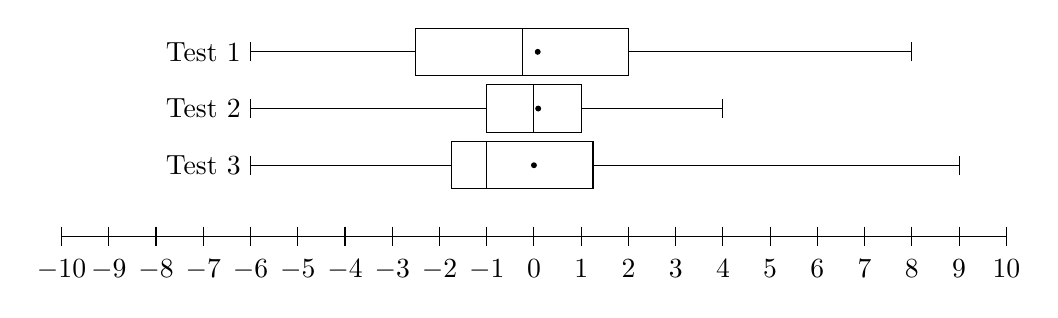
\begin{tikzpicture}[scale=0.6]
%Test 1
\draw (-2.5,3.4) rectangle (2,4.4); % Boks
\draw (-0.25,3.4) -- (-0.25,4.4); % Median streg
\draw (2,3.9) -- (8,3.9); % Fra øvre kvartil til maks
\draw (-2.5,3.9) -- (-6,3.9);% Fra nedre kvartil til min
\draw (8,3.7) -- (8,4.1); % Maksimum vertikal streg
\draw (-6,3.7) -- (-6,4.1); % Minimum vertikal streg
\node[left] at (-6,3.9) {Test 1};
\filldraw[color=black] (0.08,3.9) circle (0.05cm); % Gennemsnittet

%Test 2
\draw (-1,2.2) rectangle (1,3.2); % Boks
\draw (0,2.2) -- (0,3.2); % Median streg
\draw (1,2.7) -- (4,2.7); % Fra øvre kvartil til maks
\draw (-1,2.7) -- (-6,2.7);% Fra nedre kvartil til min
\draw (4,2.5) -- (4,2.9); % Maksimum vertikal streg
\draw (-6,2.5) -- (-6,2.9); % Minimum vertikal streg
\node[left] at (-6,2.7) {Test 2};
\filldraw[color=black] (0.09,2.7) circle (0.05cm); % Gennemsnittet

%Test 3
\draw (-1.75,1) rectangle (1.25,2); % Boks
\draw (-1,1) -- (-1,2); % Median streg
\draw (1.25,1.5) -- (9,1.5); % Fra øvre kvartil til maks
\draw (-1.75,1.5) -- (-6,1.5);% Fra nedre kvartil til min
\draw (9,1.3) -- (9,1.7); % Maksimum vertikal streg
\draw (-6,1.3) -- (-6,1.7); % Minimum vertikal streg
\node[left] at (-6,1.5) {Test 3};
\filldraw[color=black] (0.00,1.5) circle (0.05cm); % Gennemsnittet

% Linje med værdier
\draw (-10,0) -- (10,0);

% Tal på linje
\foreach \x in {-10,-9,...,10} {
	\draw (\x, 0.2) -- (\x, -0.2);
     \node[below] at (\x, -0.3) {$\x$};
}

\end{tikzpicture}
\caption{Boksplot for Test 1}
\label{kompas:boksplot}
\end{figure}

\subsubsection{Test 2 - På stabil konstruktion}
Andet forsøg blev udført med kompasset monteret på en selvstændig og langt mere stabil konstruktion, for at se om dette ville kunne forbedre resultaterne.
Disse resultater kan ses i \cref{kompas:test1:table}.

\begin{description}
\item[Største afvigelse]{6\dg}
\item[Mindste afvigelse]{0\dg}
\item[Gennemsnitlig afvigelse]{1.66}
\end{description}

\begin{table}[h]
\begin{tabularx}{\textwidth}{|>{\centering\arraybackslash}X|>{\centering\arraybackslash}X||>{\centering\arraybackslash}X|>{\centering\arraybackslash}X||>{\centering\arraybackslash}X|>{\centering\arraybackslash}X|}
\hline
\textbf{Aflæst} & \textbf{Målt} & \textbf{Aflæst} & \textbf{Målt} & \textbf{Aflæst} & \textbf{Målt} \\ \hline
0-0		& 4,5\dg	& 110-120	& 12\dg		& 296-314	& 20,5\dg \\ \hline
0-2		& 0,5\dg	& 120-146 	& 18\dg		& 314-338	& 21\dg \\ \hline
2-14	& 13\dg		& 146-160	& 15,5\dg	& 338-338	& 6\dg \\ \hline
14-32	& 22\dg		& 160-188	& 20,5\dg	& 338-340	& 0\dg \\ \hline
32-42	& 11\dg		& 188-210	& 21\dg		& 340-358	& 17\dg \\ \hline
42-68	& 29\dg		& 210-234	& 22\dg		& 358-360		& 2,5\dg \\ \hline
68-74	& 5\dg		& 234-262	& 30,5\dg	& 			& \\ \hline
74-94	& 19\dg		& 262-288	& 26\dg		& 			& \\ \hline
94-110	& 13\dg		& 288-296	& 10,5\dg	& 			& \\ \hline
\end{tabularx}
\caption{Målinger foretaget med kompas monteret på stang over ultralyds-sensor}
\label{kompas:test2:table}
\end{table}

\begin{figure}[h]
\centering
\begin{tikzpicture}[thick]
\draw(0.5,0) rectangle (2.5,1); % Boks
\draw (1.5,0) -- (1.5,1); % Median streg
\draw (2.5,0.5) -- (6,0.5); % Fra øvre kvartil til maks
\draw (0.5,0.5) -- (0,0.5);% Fra nedre kvartil til min
\draw (6,0.3) -- (6,0.7); % Maksimum vertikal streg
\draw (0,0.3) -- (0,0.7); % Minimum vertikal streg
\filldraw[color=black] (1.66,0.5) circle (0.05cm); % Gennemsnittet

% Linje med værdier
\draw (0,-1) -- (10,-1);
\draw[snake=ticks,segment length=1cm] (0,-1) -- (10,-1);

% Tal på linje
\node[below] at (0,-1.1) {$0$};
\node[below] at (1,-1.1) {$1$};
\node[below] at (2,-1.1) {$2$};
\node[below] at (3,-1.1) {$3$};
\node[below] at (8,-1.1) {$8$};
\end{tikzpicture}
\caption{Boksplot for Test 1}
\label{kompas:test1:boksplot}
\end{figure}
